\section{Retirement investments.}

\begin{enumerate}[label=\textbf{\Alph*}.]

    \item The percentage yield on an investment has a Gaussian distribution with mean of 8\% and standard deviation (SD) of 15\%. (A yield of 8\% would mean the amount of money increases by a factor of 1.08 in a year. A yield of -8\% would mean multiplying by 0.92 instead.) Suppose that you put \$3000 into a retirement account investing in this item on January 1st of every year, starting in 2018. What is the mean amount of money you will have in the account on Dec 31, 2047? Show a plot of the distribution of the amount of money on that date for 1000 trials of the ``experiment''. What is the SD? Hand in your code or equivalent documentation.

    I did this computationally, here are the results:

    Value on Dec 31, 2047: 370000

    Standard deviation: 228000

    \todo[inline]{how to deal with dec 31st vs jan 1?}

    \begin{figure}[H]
        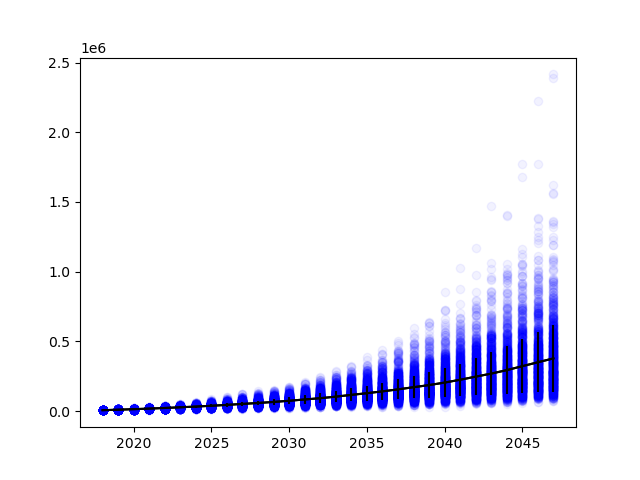
\includegraphics[width=\textwidth]{q4_a.png}
    \end{figure}

    \item Suppose now that the retirement account contains three classes of investments: Canadian stocks, foreign stocks, and bonds. The yields on these three investments each vary randomly but with some correlation. Here is the yield information for each investment: $\mu_C = 8\%, \sigma_C = 15\%, \mu_F = 8\%, \sigma_F = 15\%, \mu_B = 5\%, \sigma_B = 7\%, \rho_{CF}=0.50, \rho_{CB}=0.20, \rho_{FB}=0.05$. On January 1 of each year you put \$1000 into each class of investment. Show the distribution of the total amount of money in your account on Dec 31, 2047. What are the mean and SD?

    Let's do this computationally again, but first let's explain some mystery numbers that will appear in the code, using the hint in the question.

    \begin{align*}
        C &= \mathcal{N}(\mu = 0.08, \sigma = 0.15)
    \end{align*}

    Then define a linear combination of $C$ and $F$ in terms of another Gaussian:
    \begin{align*}
        Y &= C - F \\
    \end{align*}

    $Y = \mathcal{N}(\mu=0, \sigma_Y=\sigma_C)$.

    Check this works out:
    \begin{align*}
        \operatorname{Var}(Y) &= 1^2 \operatorname{Var}(C) + 1^2 \operatorname{Var}(F) - 2\operatorname{Cov}(C,F) \\
        \operatorname{Var}(Y) &= \sigma_C^2 + \sigma_F^2 - 2\rho_{CF}\sigma_C\sigma_F \\
        \sigma_C^2 &= \sigma_C^2 + \sigma_C^2 - 2\frac{1}{2}\sigma_C^2 \\
        \sigma_C^2 &= \sigma_C^2 \\
    \end{align*}

    \begin{align*}
        \mu_Y &= \mu_C - \mu_F = 0 \\
    \end{align*}

    So to generate $F$ we can use this:
    \begin{align*}
        F &= C - Y, Y = \mathcal{N}(\mu=0, \sigma=\sigma_C) \\
    \end{align*}

    Then to generate $B$, consider another combination: $Q = aY + bB$

    \begin{align*}
        \mu_Q &= a\mu_Y + b\mu_B \\
        \mu_Q &= a(0) + b(0.05) \\
        \mu_Q &= b(0.05) \\
    \end{align*}

    Let $b=1$ for simplicity.

    \begin{align*}
        \operatorname{Var}(Q) &= a^2 \operatorname{Var}(Y) + \operatorname{Var}(B) + 2ab\operatorname{Cov}(Y,B) \\
        &= a^2 (0.15)^2 + (0.07)^2 + 2a(\operatorname{Cov}(C,B) - \operatorname{Cov}(F,B)) \\
        &= a^2 (0.15)^2 + (0.07)^2 + 2a(\rho_{C,B}\sigma_C\sigma_B - \rho_{F,B}\sigma_F\sigma_B) \\
        &= a^2 (0.15)^2 + (0.07)^2 + 2a((0.20)(0.15)(0.07)- (0.05)(0.15)(0.07)) \\
        &= a^2 (0.15)^2 + (0.07)^2 + 0.00315 a \\
    \end{align*}

    We still have a free parameter, let $a=1$
    \begin{align*}
        \sigma_Q^2 &= (0.15)^2 + 0.00315 + (0.07)^2\\
        \sigma_Q &= 0.174785583 \\
    \end{align*}

    (there's some round-off error here but I assume it's small enough we can ignore it)

    So $Q = Y + B, Q = \mathcal{N}(\mu=0.05, \sigma=0.174785583)$.


    Results:

    Value Dec 31, 2047: 204918.0565428472

    Standard deviation: 102948.69611667504

    Plot of our results:
    \begin{figure}[H]
        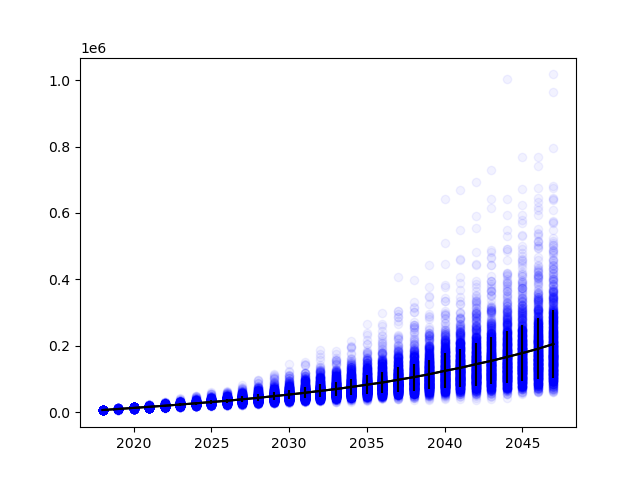
\includegraphics[width=\textwidth]{q4_b.png}
    \end{figure}

    \item Now suppose we add a procedure called ``rebalancing''. On January 1 of each year we contribute a total of \$3000 to the account, but at the same time we redistribute the total amount of money in the account evenly between the three investments. How does this change the total amount on Dec 31, 2047? Show a plot of the distribution, and report the mean and SD as well.

    Value Dec 31, 2047: 119628.72535169181

    Standard deviation: 45756.874877228125

    Plot of results:
    \begin{figure}[H]
        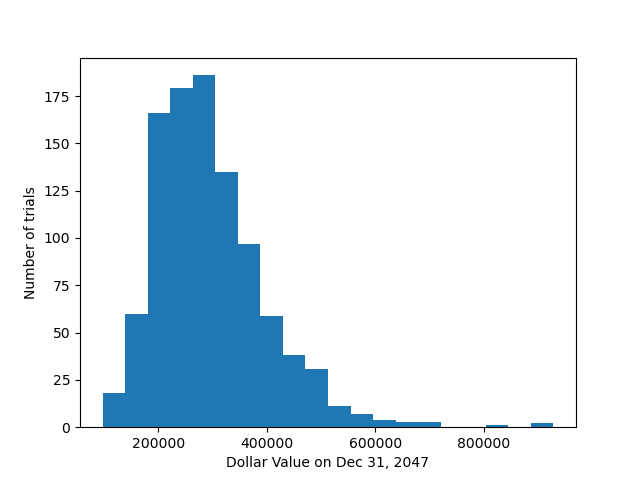
\includegraphics[width=\textwidth]{q4_c.png}
    \end{figure}

    \todo[inline]{This feels kinda sussy, why is everything so much lower? Was there another constraint we could have used? Also this looks linear rather than exponential...}


\end{enumerate}

